\section{The \instname\ data reduction flow.}
\label{sec:reduction_flow}

FORS is the visual and near-UV FOcal Reducer and low dispersion Spectrograph for the Very Large Telescope (VLT) of the European Southern Observatory (ESO). Two versions of FORS have been built and mounted at the VLT, but in April 2009, FORS1 was removed to make room for X-shooter, so only FORS2 is now in operation.
FORS is designed as an all-dioptric instrument for the wavelength range from 330 nm to 1100 nm and provides an image scale in the standard mode of 0.25 arc sec per pixel with the readout mode (2×2 binning).

FORS2 offers three spectroscopic modes: long-slit spectroscopy (LSS) using a mask with $6.8^{'}$ long slits of
different widths, and multi-object spectroscopy with movable slit blades (MOS, slit length about $20^{''}$) and with masks (MXU, arbitrary slit length, curved and tilted slits possible). The spectrophotometric standard stars for flux calibration are always taken in MOS mode, where the slitlets are used to create a long slit of $5^{''}$ width at the position of the long-slit used for the science data or at the center of the field-of-view for multi-object
spectroscopy. 

FORS2 has several volume-phase holographic grisms, for which the response depends on the position on the CCD. This requires specific steps during the flux calibration, which are handled correctly by the pipeline.

The Longitudinal Atmospheric Dispersion Corrector corrects the effects of atmospheric refraction up to an airmass of about 1.5, thereby enabling observations with arbitrary angles on sky without flux losses due to
atmospheric refraction.

The FORS2 supports the correction of telluric absorption using the molecfit algorithm.

This document describes reduction of the data taken in any of the spectroscopic modes of FORS1 and FORS2 (for simplicity, the instrument is often addressed as FORS). It does not cover the other modes, which are described in different tutorial documents.



The overall data flow of the \instname\ pipeline is displayed in Figure \ref{fig:reduction_cascade}.

 
\begin{figure}[h!]
\centering

\includegraphics[width=0.9\textwidth]{../instrument_tutorial/figures/reduction_cascade.jpg}
\caption{The data reduction cascade of the \instname\ workflow.}
\label{fig:reduction_cascade}
\end{figure}



The reduction cascade is organized in tasks, which represent
well-defined steps in the process. Tasks can be grouped inside
sub-workflows.  Each task runs a recipe; the detailed description of
the algorithms, input, outputs and recipe parameters used in each
recipe are available in the pipeline manual. Here, we present only the
description of most important features.

The \wkfname\  \edps\ workflow is designed to execute the tasks that
deliver the final reduced data cube for each dataset. It can be either
the product of a single exposure, or the combination of multiple
exposures. Only calibrations needed by the selected the scientific
exposures are processed.

It is possible to set \edps\ to perform the data reduction until a
certain step of the reduction chain (e.g. to reduce only standar
stars, or only flat fields).  This is done by specifying the desired
tasks in the field {\bf Select reduction target} of the {\bf Raw Data}
tab.

The reduction steps of the \wkfname\ workflow are listed below. Before
starting the reduction, the parameters of the recipes associated to
each task can be configured by pressing the button

\includegraphics[width=0.8cm]{../common/figures/configure_dataset.jpg}
close to each dataset configuration.
See for more info on the configuration editor \ref{sec:configuration_editor}



\subsection{Create Master Bias}

Task: {\bf bias} Recipe: {\bf fors\_bias}

In this step the combined MASTER\_BIAS is produced out of the input raw frames. The bias raw frames are acquired with an exposure time of 0 seconds and a closed shutter. They thus record only the signal
that is added during the read-out of the CCD to avoid negative numbers. A sequence of 5 or 20 bias frames is taken the day following the observations as part of the FORS2 calibration plan (the calibration plan was changed in November 2014; Since then, 20 instead of 5 bias frames are taken per setting).
Using the full bias frame instead
of just the pre-overscan allows the user to correct for potential offsets between the bias level on the detector and the pre-overscan regions.

The same MASTER\_BIAS product per setup is further used in reduction of the LSS, MOS and MXU data.

Figure \ref{fig:examining_products} demonstrates how the pipeline products can be examined on the example of the product of the task: {\bf bias}, recipe {\bf fors\_bias}. Further, the Figure \ref{fig:master_bias} displays an example of the quality plot for the MASTER\_BIAS. The image should be uniform, without visible flux gradient. You can also display another extension, IMAGE.ERR containing estimated error per pixel. See Section \ref{sec:configuration_bias} for more information on how to improve the product if needed.


\begin{figure}[h!]
\centering
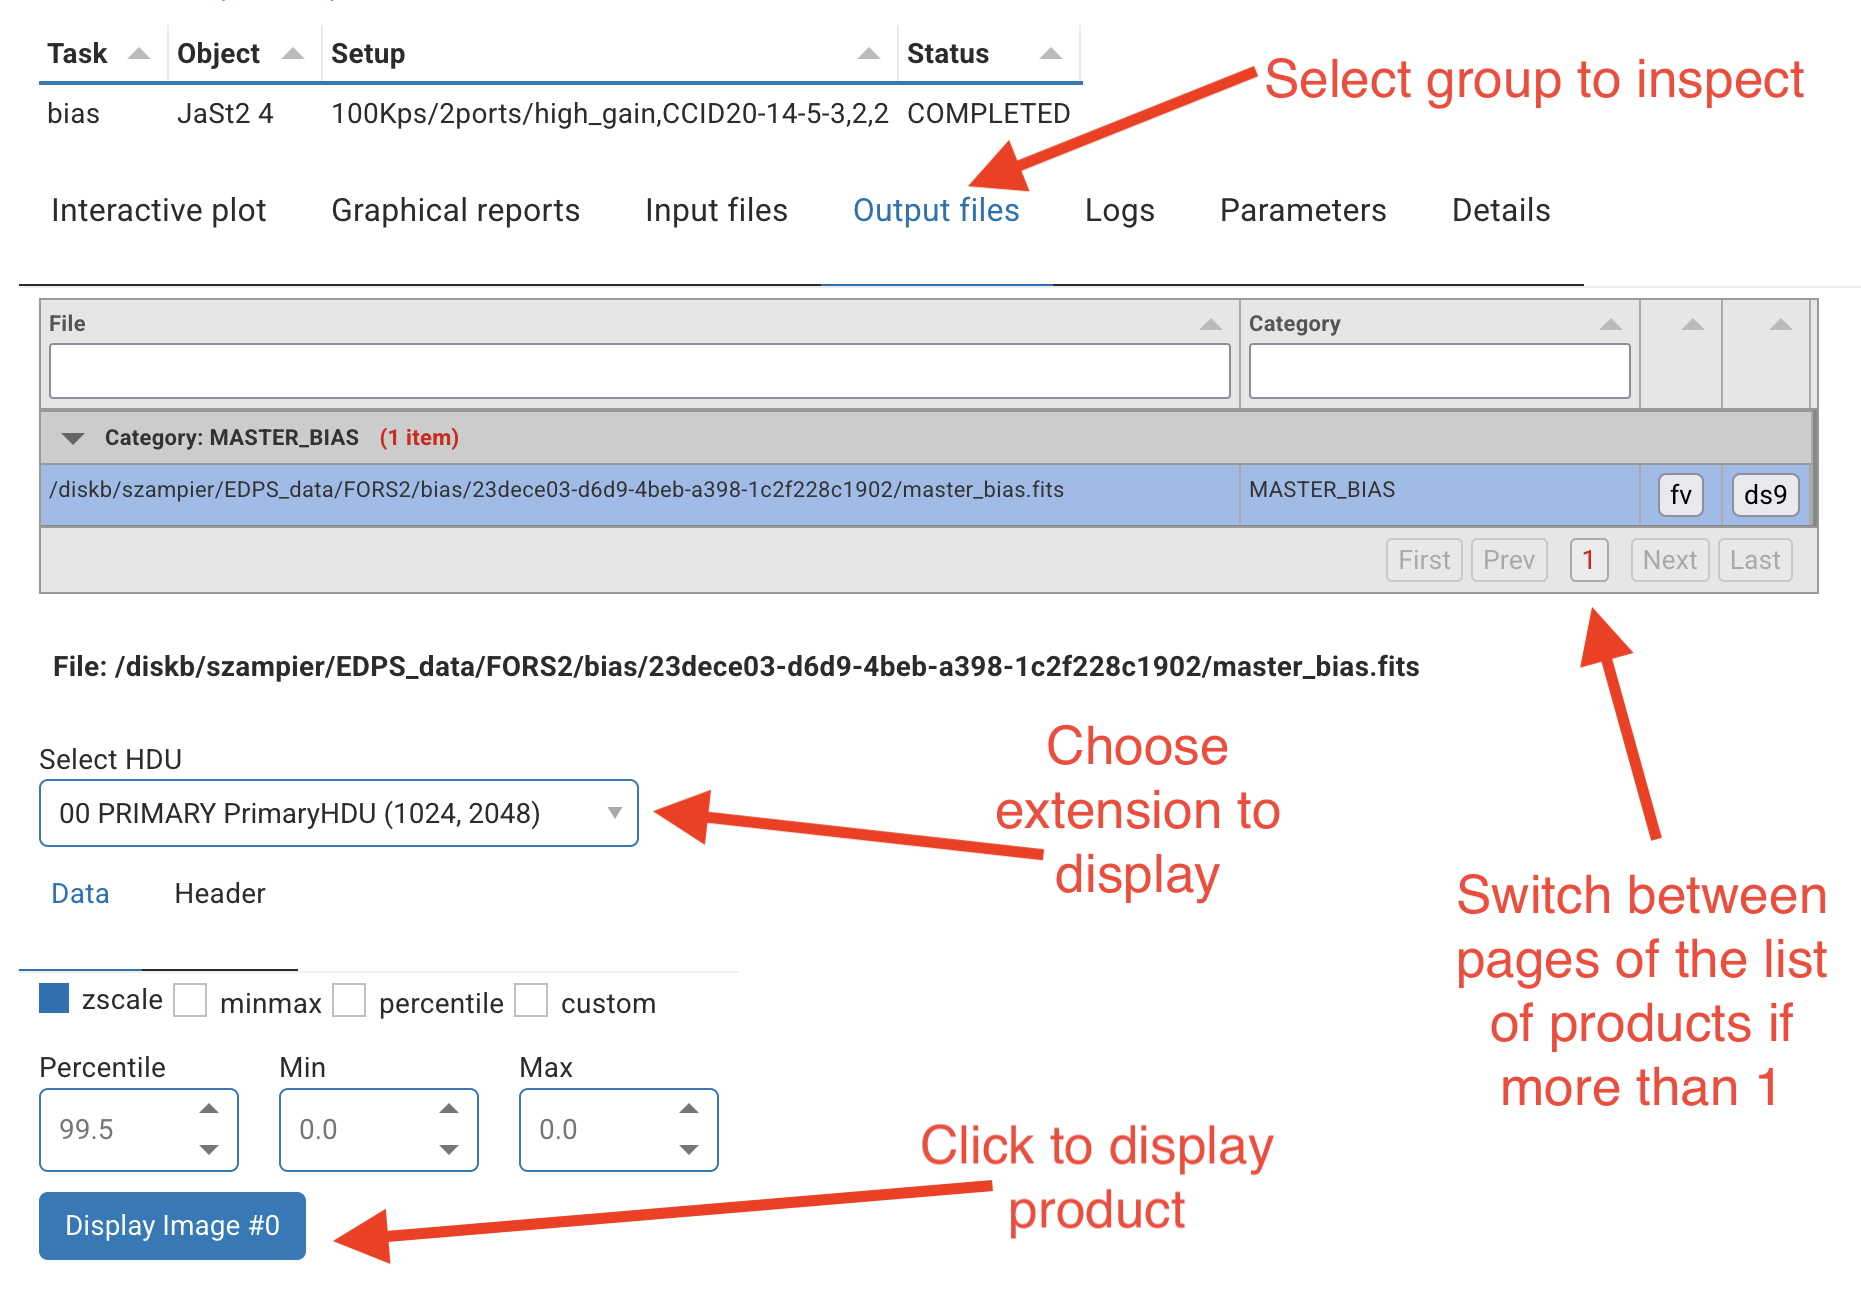
\includegraphics[width=0.9\textwidth]{../instrument_tutorial/figures/examining_products.jpg}
\caption{Examining product of the task: {\bf bias}, recipe: {\bf fors\_bias}. }
\label{fig:examining_products}
\end{figure}

\begin{figure}[h!]
\centering
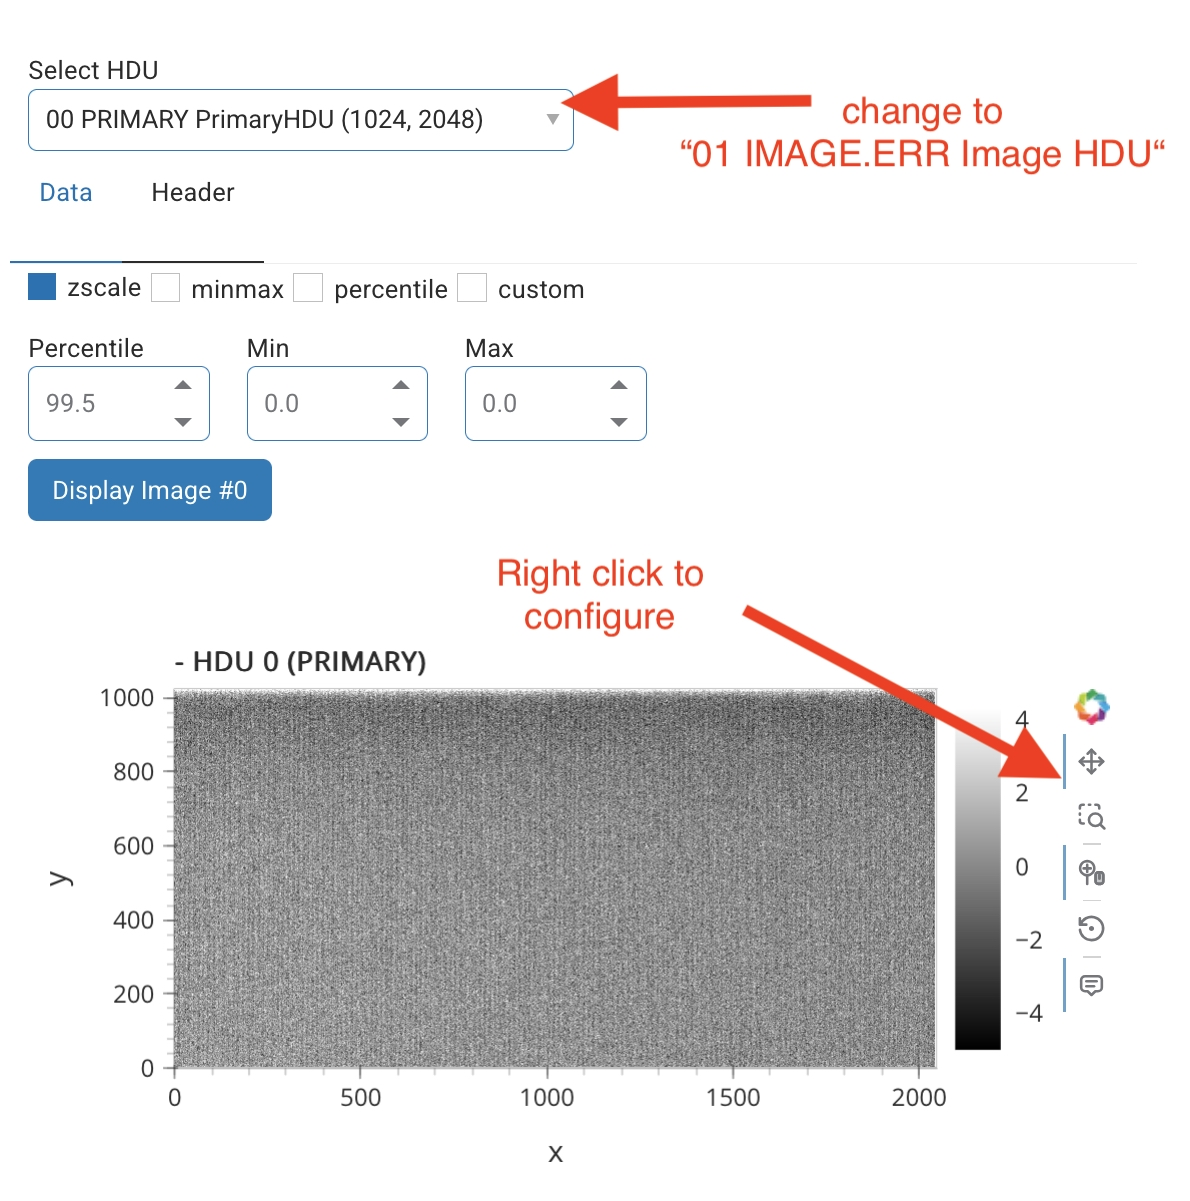
\includegraphics[width=0.9\textwidth]{../instrument_tutorial/figures/master_bias.jpg}
\caption{The quality plot of the MASTER\_BIAS. }
\label{fig:master_bias}
\end{figure}


\subsection{Create Master Flat Field, Dispersion Solution and Correction for Spatial Distortion}

Tasks: {\bf calibration\_lss}, {\bf calibration\_mos}, {\bf calibration\_mxu}, {\bf calibration\_std}  Recipe: {\bf fors\_calib}

In one step, the input screen flat raw calibration frames: SCREEN\_FLAT\_LSS/MOS/MXU together with the arc lamp raw frame: LAMP\_LSS/MOS/MXU
are used to create a normalized master flat-field, a 2D dispersion solution, correction for spatial distortion, and to determine the slit limits.

The exposure of the arc lamp(s) He, HgCd, and Ar (at the lowest spectral resolution with grism 150I) and in addition the Ne lamp (at higher resolution) are acquired together with the screen flat field data to ensure that they are all recorded at the same mask position. 

The task {\bf calibration\_std} produces similar master calibrations used to process spectrophotometric standard star data - the 5 arcsec slit width MOS observations.

The tasks {\bf calibration\_hc\_lss} and {\bf calibration\_hc\_std} also run the {\bf fors\_calib} recipe but only reduce the FORS spectroscopic calibration data used for monitoring.


Main Products:

Not all output frames listed here are always produced. Some are never created in case of LSS or LSS-like data. The LSS-like data are obtained in the MOS instrument mode when all the slits are aligned. This kind of data are processed as a single
long slit spectrum. The product categories will contain the acronym LONG before the instrument mode tag: for instance, DELTA\_IMAGE\_MOS will become DELTA\_IMAGE\_LONG\_MOS.

\begin{itemize}

\item MASTER\_SCREEN\_FLAT\_LSS/MOS/MXU - master screen flat field (for verification only); comparing it to the normalized master flat allows to see if all slitlets for MOS/MXU have been found

\item MASTER\_NORM\_FLAT\_LSS/MOS/MXU - normalized master flat field, derived by dividing the master screen flat by its smoothed version 

\item DISP\_COEFF\_LSS/MOS/MXU - table containing the wavelength calibration polynomial coefficients

\item DISP\_RESIDUALS\_LSS/MOS/MXU - residuals of each wavelength calibration fit (in pixels)

\item DISP\_RESIDUALS\_TABLE\_LSS/MOS/MXU - table containing different kinds of residuals of a sample of wavelength calibration fits

\item FLAT\_SED\_LSS/MOS/MXU - image containing the spectral energy distribution of the flat; each image row corresponds to the SED (Spectral Energy Distribution) of one slit ordered as in the SLIT\_LOCATION\_MXU table; the SED profile is wavelength calibrated using the polynomial of the central row of the illuminated region

\item SLIT\_LOCATION\_LSS/MOS/MXU - table containing the slit positions on the CCD and on the reduced lamp image

\item WAVELENGTH\_MAP\_LSS/MOS/MXU - wavelength map image with the same size as the CCD, where each pixel is assigned the value of the wavelength at its center

\item SPATIAL\_MAP\_MOS/MXU - spatial map image (MOS/MXU only), which has the
same size as the CCD, where to each pixel is assigned the value of its
distance (in CCD pixels) from the top edge of the spectrum it belongs to

\item SPECTRAL\_RESOLUTION\_LSS/MOS/MXU - spectral resolution table containing the mean spectral resolution for each reference arc lamp line

\item CURV\_COEFF\_MOS/MXU - table (MOS/MXU only) containing coefficients of the polynomials used to fit the spectral curvature

\item CURV\_TRACES\_MOS/MXU - table (MOS/MXU only) containing the y CCD positions of the detected spectral edges

\item REDUCED\_LAMP\_LSS/MOS/MXU - reduced lamp image (for verification
only), i.e. rectified and wavelength calibrated arc lamp image. This
is the result of applying the extraction mask derived from the flat
field and arc lamp exposures to the input arc lamp exposure
itself. This image is useful to get an immediate feeling of the
goodness of the computed extraction mask.

\item DELTA\_IMAGE\_LSS/MOS/MXU - deviation from the linear term of the wavelength calibration polynomials

\end{itemize}

In this step, few properties of the master calibrations should be checked : quality of the wavelength calibration, distortion correction (not applicable to LSS and LSS-like data), the flat field combination and normalization. It is recommended to create and inspect "Graphical reports" (for "Both" "Raw data" and "Reduced data") and the "Output files" links among the quality plots.

\begin{figure}[h!]
\centering
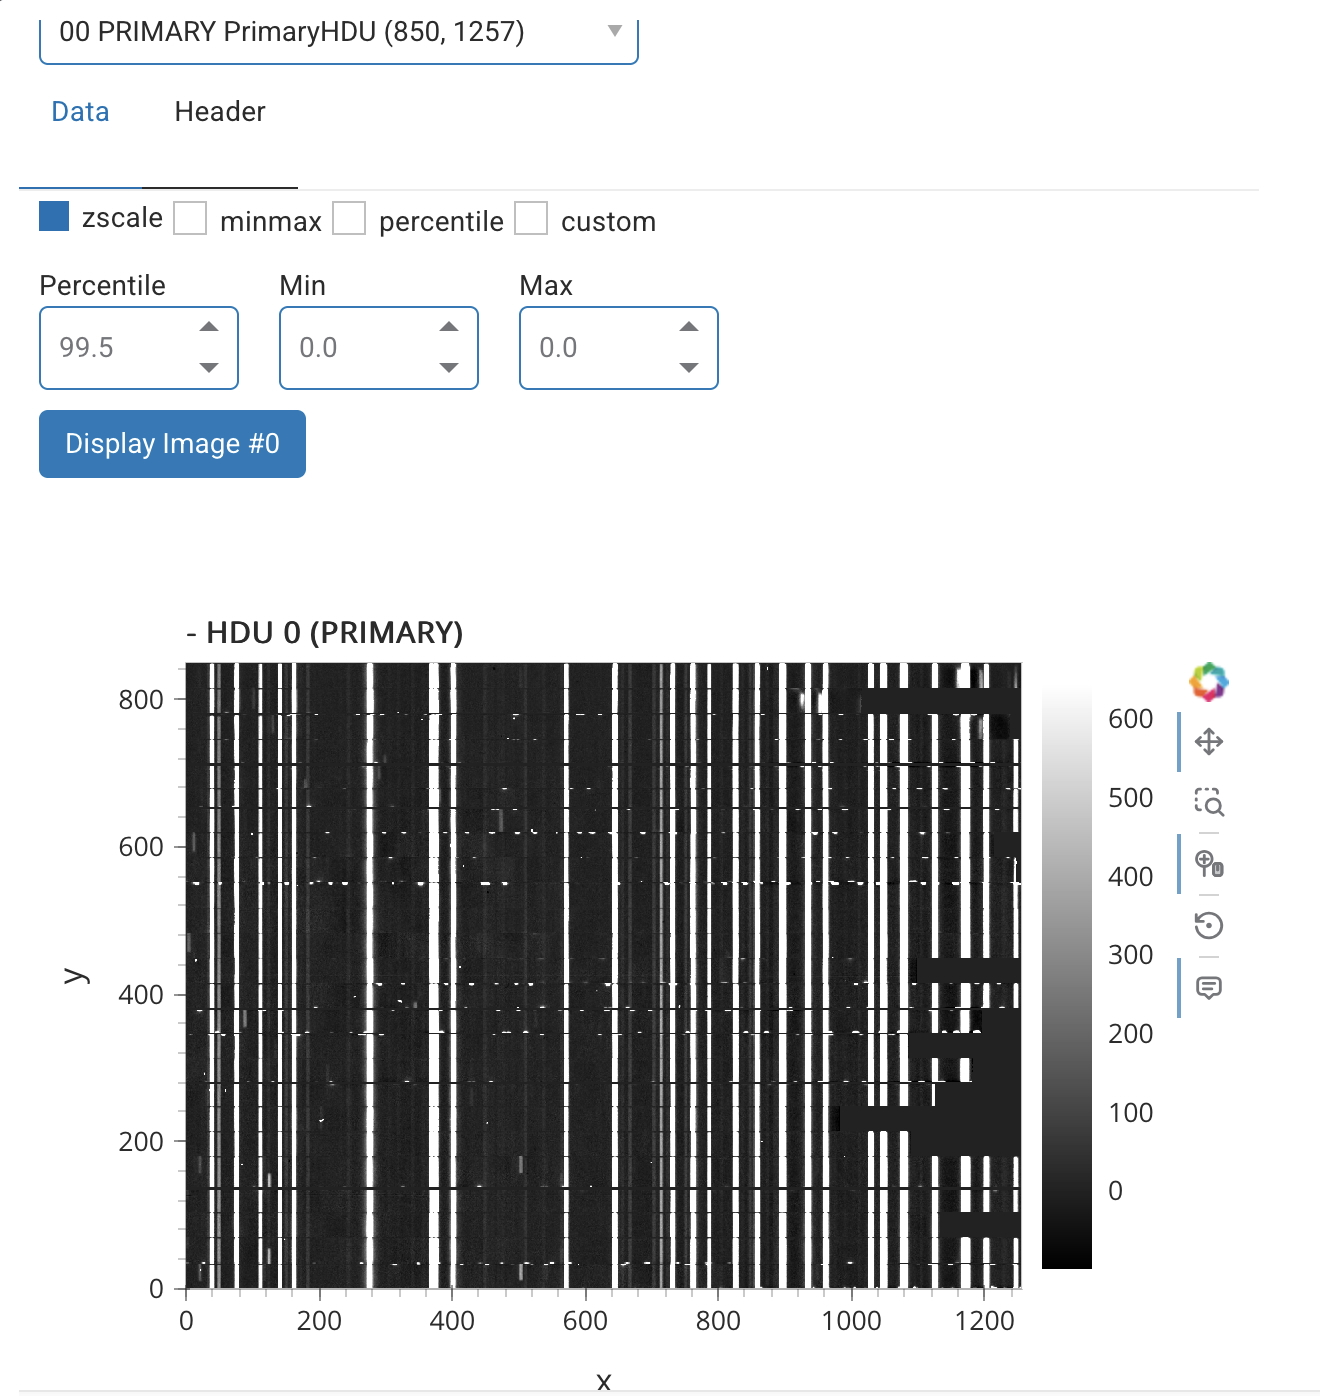
\includegraphics[width=0.9\textwidth]{../instrument_tutorial/figures/reduced_lamp_mxu.jpg}
\caption{Example of the quality plot of the REDUCED\_LAMP\_MXU product of the task: {\bf calibration\_mxu}, recipe: {\bf fors\_calib}. }
\label{fig:reduced_lamp_mxu}
\end{figure}

\begin{figure}[h!]
\centering
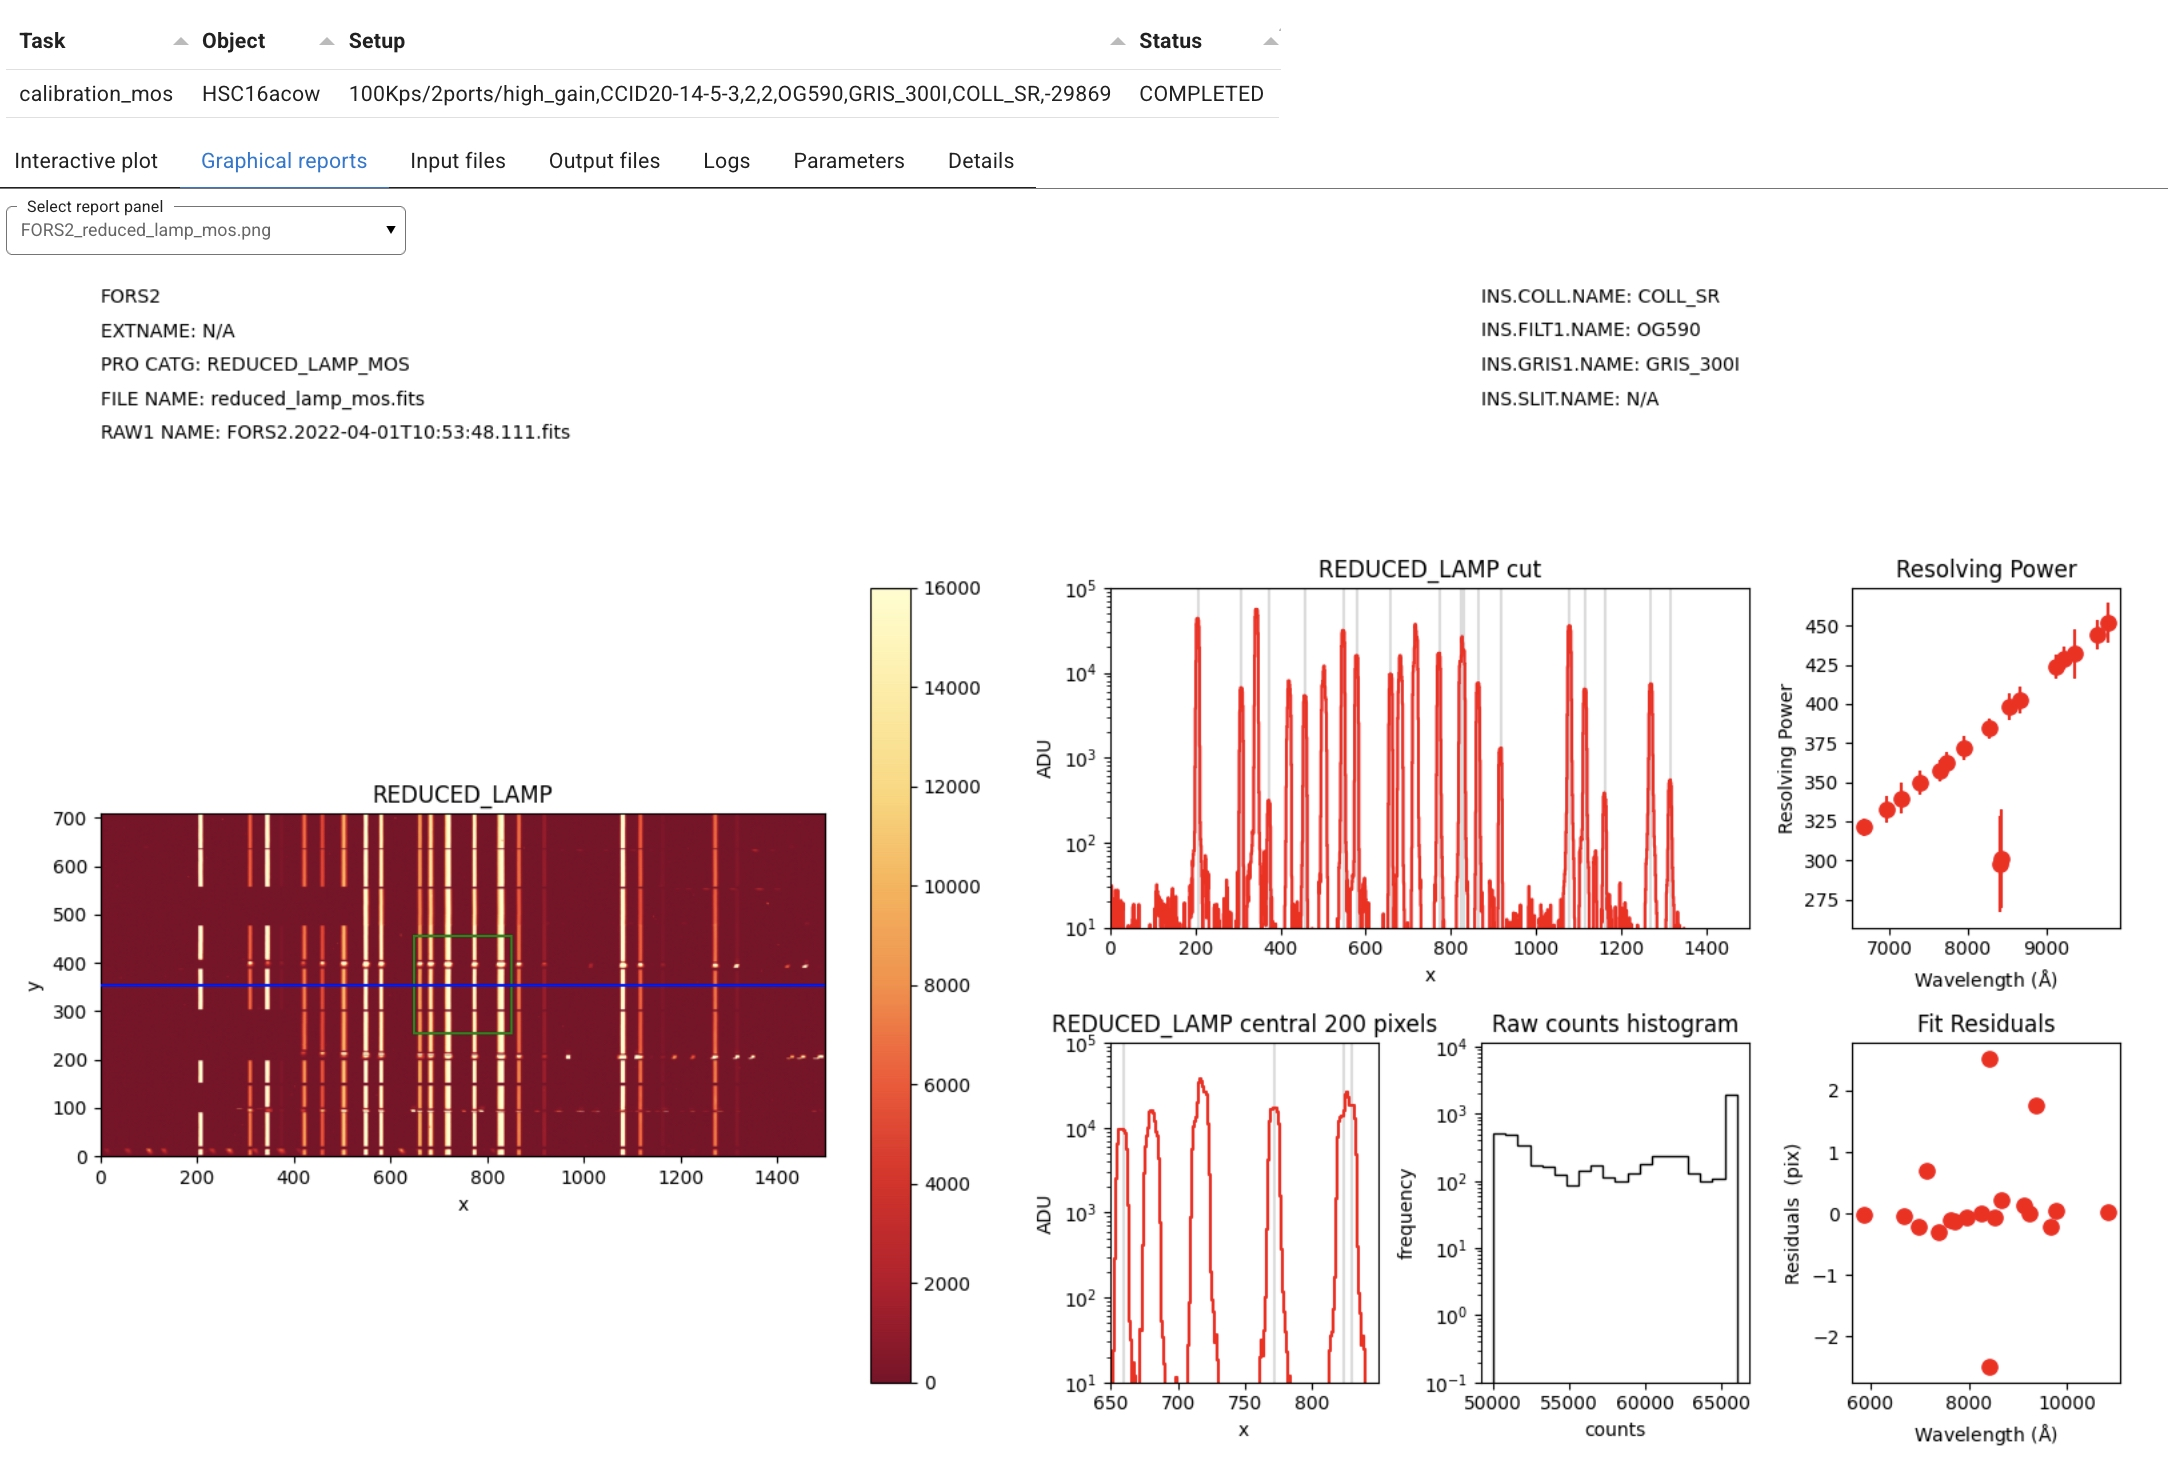
\includegraphics[width=0.9\textwidth]{../instrument_tutorial/figures/reduced_lamp_mos.jpg}
\caption{Example of the "Graphical Report" for the task: {\bf calibration\_mos}, recipe; {\bf fors\_calib} reduced\_lamp\_mos.png. }
\label{fig:reduced_lamp_mos}
\end{figure}

Figure \ref{fig:reduced_lamp_mxu} shows an example of the wavelength-calibrated arc lamp frame (REDUCED\_LAMP\_MXU product), while Figure \ref{fig:reduced_lamp_mos} the example of the "Graphical report" FORS\_reduced\_lamp\_mos. In these plots the arc lamp lines should run straight from top to
bottom without any empty rows between them. Particular attention should be given to lines at the blue and red ends of each spectrum, where the polynomial fit is more sensitive to small variations of the signal. Some arc lines may show gaps due to the placement of the slitlets, but empty rows without any lines point towards problems with the detection of the arc lamp lines. For LSS and LSS-like data the arc lines extend from top to bottom without any slitlet marks.

Residuals between predicted and detected arc line position (the DISP\_RESIDUALS\_LSS/MOS/MXU product) should generally be below 0.5 pixel. If they show systematic variations the polynomial degree used to fit the dispersion relation may be too low (or in rare cases too high). If the scatter appears very large one should zoom in, because there are often only a few outliers and the majority of the residuals are within ±0.5 pixels. 

The spatial map (SPATIAL\_MAP\_MOS/MXU product) has as pixel values the distance of a pixel from the bottom of the
respective slitlet. The regions of the slitlets should not be strongly curved nor should regions of different slitlets overlap with each other.


\begin{figure}[h!]
\centering
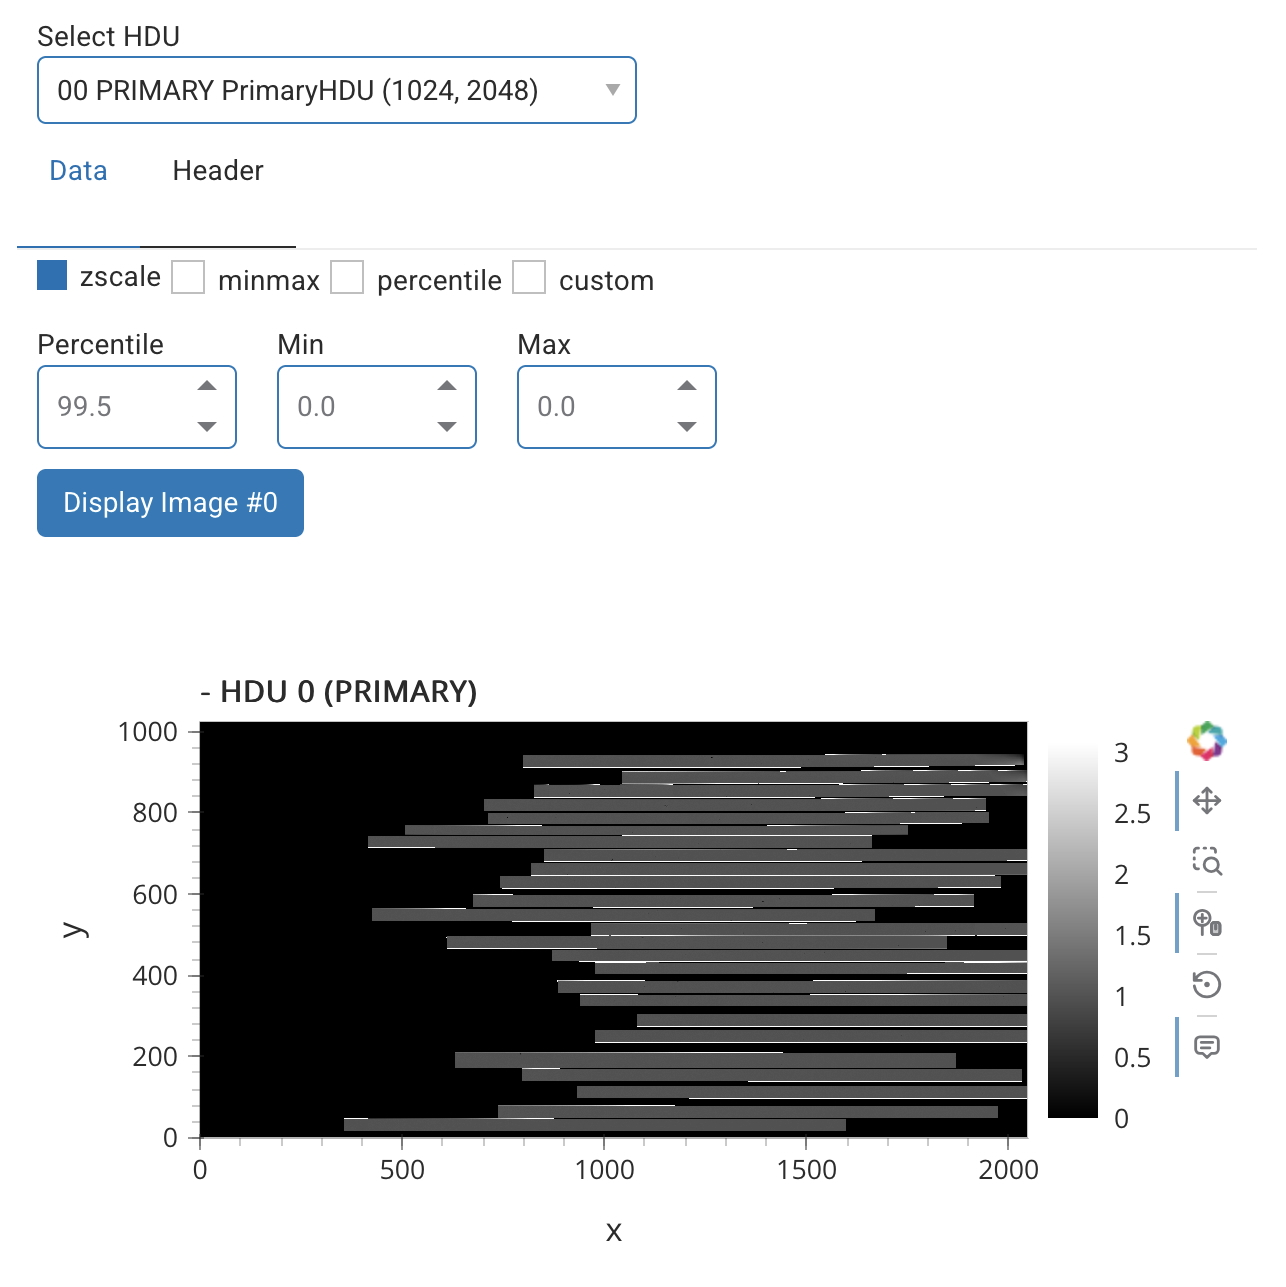
\includegraphics[width=0.9\textwidth]{../instrument_tutorial/figures/master_norm_flat_mxu.jpg}
\caption{Example of the quality plot of the MASTER\_NORM\_FLAT\_MXU product of the task: {\bf calibration\_mxu}, recipe: {\bf fors\_calib}. }
\label{fig:master_norm_flat_mxu}
\end{figure}

Figure \ref{fig:master_norm_flat_mxu} shows an example of the MASTER\_NORM\_FLAT\_MXU product. The master flat should have the same number of slitlets as the first raw flat and their areas should also be identical.
All slitlets should be detected and there should be no spurious detections (e.g. one slitlet detected as several). For LSS and LSS-like data the illuminated region along the y-axis has to be identical between
the REDUCED\_LAMP\_LSS and the MASTER\_NORM\_FLAT\_LSS. Otherwise part of the exposed area is lost.
In the frame, depending on the normalization method residual gradients may be validly present (e.g. for {\tt sradius:} $-1$ as recommended for LSS data).

See Section \ref{sec:configuration_calibration} for more information on how to improve the products if needed.


\subsection{Compute Response Function}

Tasks: {\bf standard\_lss}, {\bf standard\_mos}   Recipes: {\bf fors\_science}

The observed spectrophotometric standard stars are stars with a well known flux distribution. They are usually observed during twilight within ±3 days of the science data.
The data are processed to create the instrument response curves. They may be later used to flux-calibrate science data in case there is no master
response curve determined for the particular grism (affects mostly
observations before January 1, 2025. After that date, the master
response curves exist for most of the grisms). The recipe
{\bf fors\_science} integrates the observed flux, corrected for gain,
exposure time and atmospheric extinction, over the intervals indicated
in the STD\_FLUX\_TABLE corresponding to the observed star (the {\tt HIERARCH ESO OBS TARG NAME} keyword is matched between the observation and the entries in the table).
The reference flux values for the star are then divided by the integrated observed flux values to create the so-called raw response. Features like strong stellar lines or regions of telluric absorption are
masked before a polynomial or a spline fit is performed to define the final response curve. 


Product:
\begin{itemize}
\item SPECPHOT\_TABLE - table with efficiency and response curves. It can be used as an input to the {\bf fors\_science} recipe when the flux-calibrated products are created.

\end{itemize}

\begin{figure}[h!]
\centering
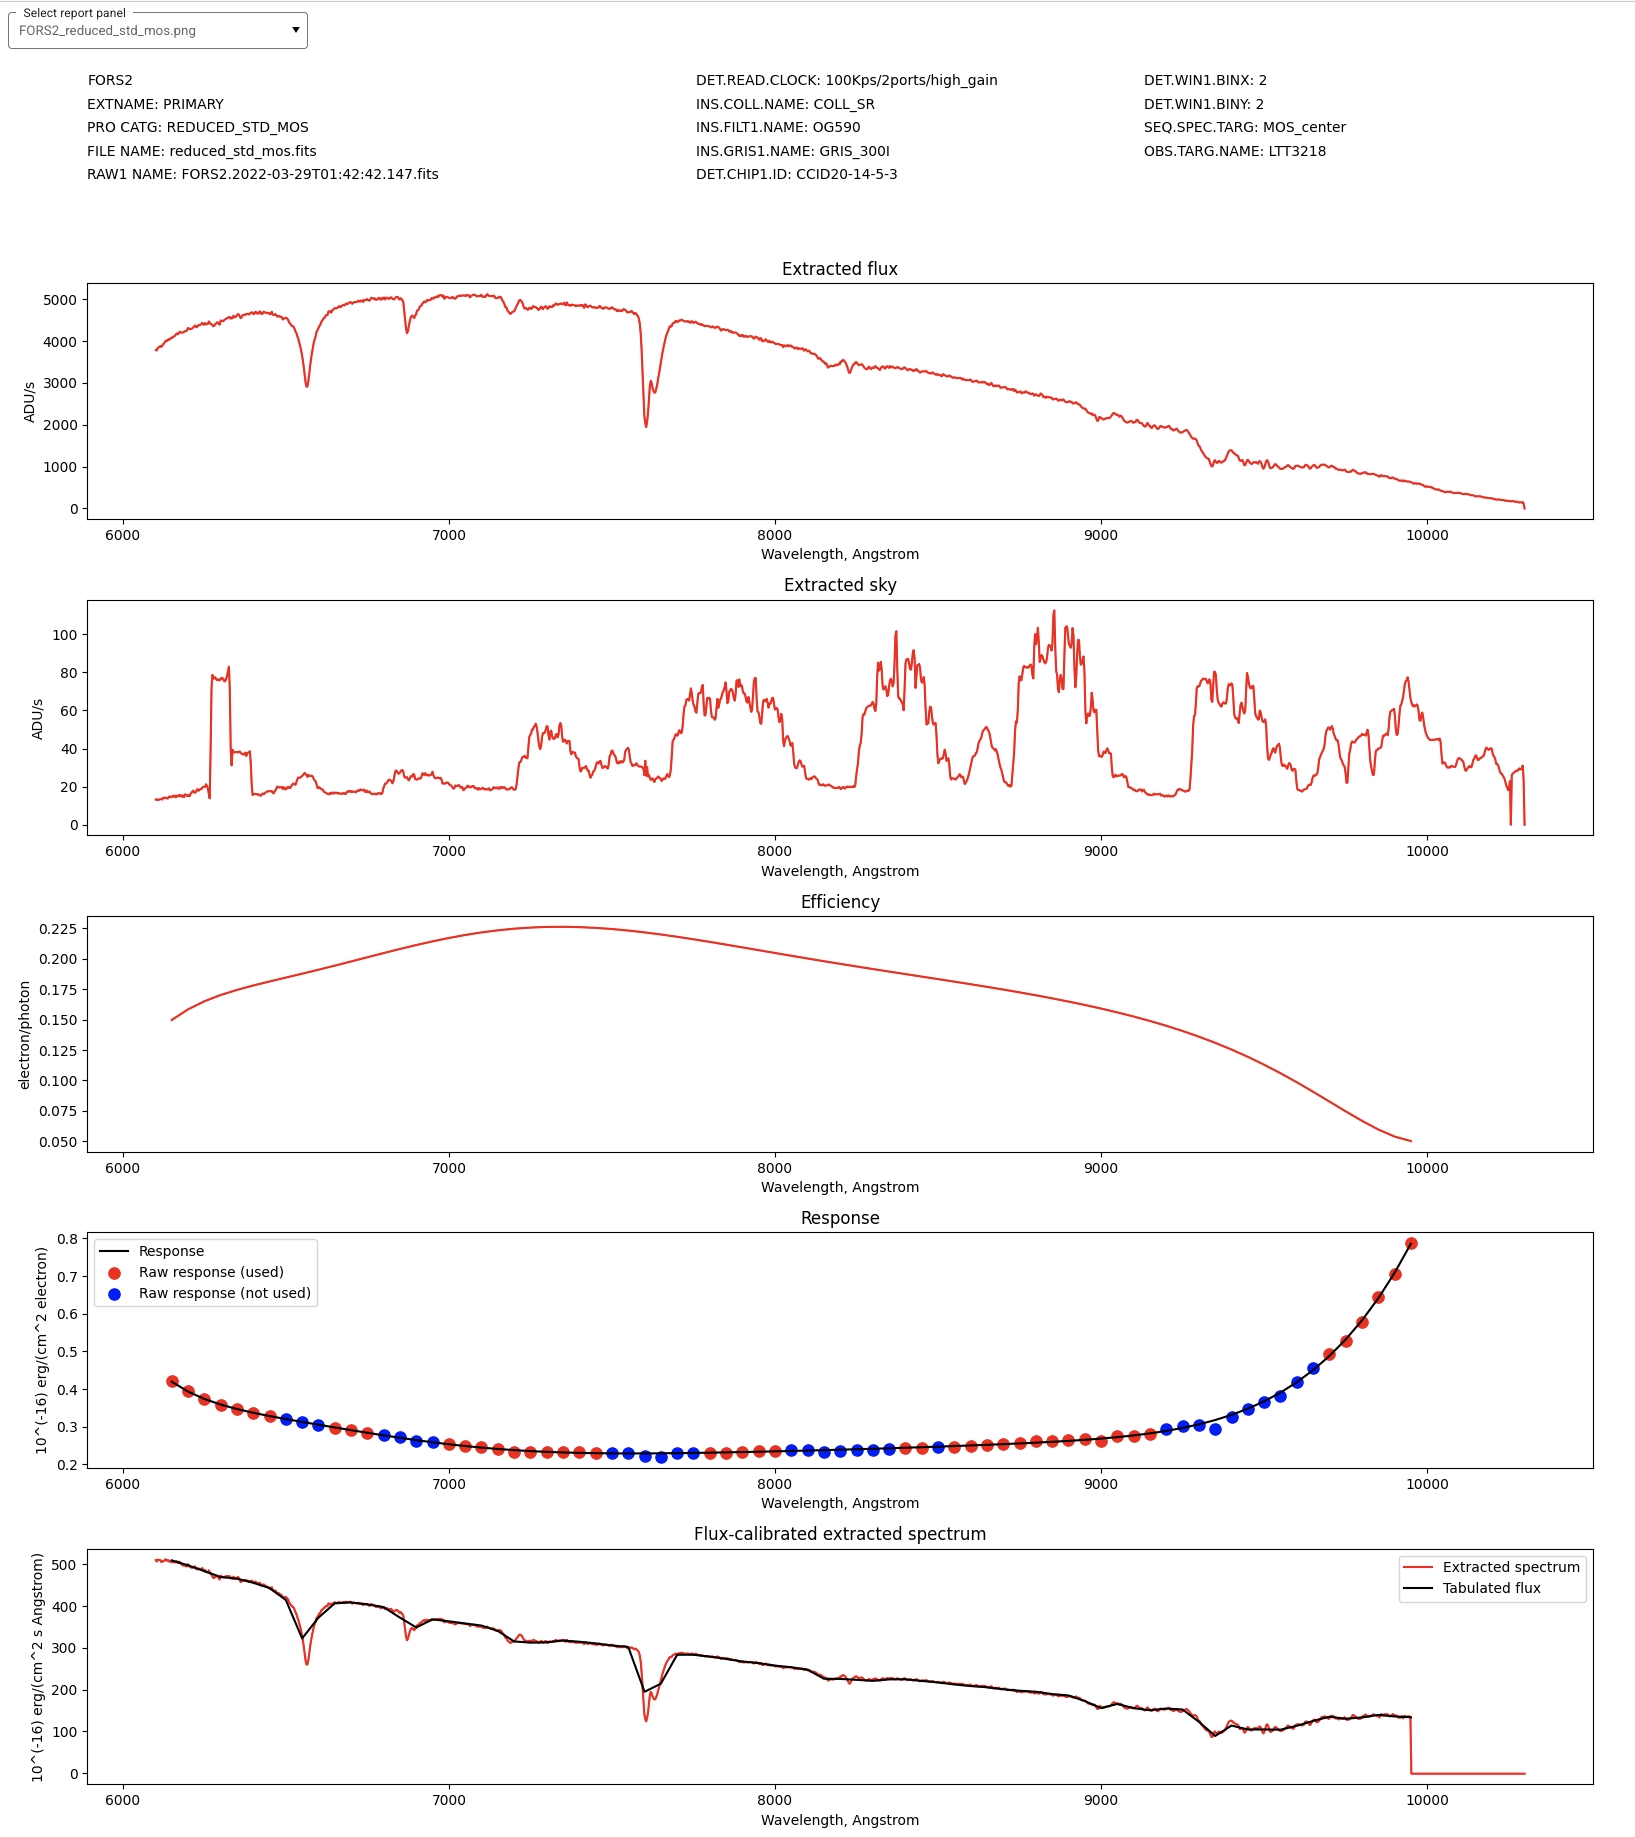
\includegraphics[width=0.9\textwidth]{../instrument_tutorial/figures/reduced_std_mos.jpg}
\caption{Example of the "Graphical report" reduced\_std\_mos.png of the task: {\bf standard\_mos}, recipe: {\bf fors\_science}. }
\label{fig:reduced_std_mos}
\end{figure}

In this step, the quality of the response curve fit should be checked.

Figure \ref{fig:reduced_std_mos} is an example of the created "Graphical report" for the relevant task: {\bf standard\_mos}, recipe: {\bf fors\_science}. The extracted standard star spectrum should show no jumps or sky emission lines. Strong gradients due to order separating filters are valid but may cause problems with the fit of the response curve.

In the "Response" panel, the dots show the raw response (ratio of reference spectrum and observed spectrum integrated over same bins as reference spectrum) and the blue line shows the corresponding fit. Blue dots are masked and not used for the fit.

In the bottom panel the red line marks the observed standard star
spectrum calibrated with its own response curve and the black curve indicates the reference data (blue points were masked during the fitting of the response). Differences between the black and
the red lines indicate a problem with the flux calibration, usually features on a scale smaller than the bins
of the reference data. Differences between the red and black curves may indicate problems with inter- and/or extrapolation, but may also be valid, for instance due to different amounts of telluric absorption or
to differences in resolution between the reference spectra and the observed data.

Raw and fitted response - the blue curve (fit) should follow the red curve (unmasked raw response) closely. If the fit deviates from the data in the masked regions in unexpected ways (blue dots) the user may try to remove {\tt stellar\_absorption} and/or {\tt telluric} from the parameter {\tt resp\_ignore\_mode} and mask only smaller regions via {\tt resp\_ignore\_points}. Alternatively or in addition one may change the fit method and/or degree via {\tt resp\_fit\_degree} (polynomial degree) or {\tt resp\_fit\_nknots} (number of spline knots).
One should keep in mind that interpolating across a larger region (e.g. covered by telluric lines) provides at best a probable response curve, but may also show strong deviations. This is even more true for extrapolations, e.g. if a response curve has telluric regions at its edges.

Flux-calibrated standard star spectrum should
coincide with the tabulated standard star flux (blue dots were ignored during the response fit). Deviations at the very blue end may results from problems with atmospheric extinction and deviations at wavelengths above 6000 Å may point to problems with telluric absorption.

Keep in mind that occasionally there may be no STD\_FLUX\_TABLE associated to the observations of a flux standard star.


\subsection{Reduce Science Data}

Task: {\bf science\_spectra}   Recipe: {\bf fors\_science}

In this task the recipe {\bf fors\_science} is run to apply sky subtraction
and extract the spectra. The science observations get flux calibrated using the master response curve (preferred if available) or the instrument response curve derived from the standard star observation.
If neither standard star observation nor master response curve is available, then the science observation will not be flux-calibrated.

Products (the filenames for the other modes are similar but with the MOS suffix replaced by MXU, LONG\_MOS or LSS as appropriate):

{\bf 1-dimensional extracted spectra (Phase3 compliant)}

\begin{itemize}
\item REDUCED\_IDP\_SCI\_MOS - flux-calibrated spectra
\item SCI\_MOS\_TELLURIC\_CORR - flux-calibrated spectra, corrected for telluric absorption. The first extension is identical to the corresponding REDUCED\_IDP\_SCI\_MOS product, the second extension contains information on the telluric correction parameters, and the
third extension provides the telluric corrected spectrum (column {\tt cflux}). Please note that the wavelength in the third extension (column {\tt lambda}) is in $\mu$m, not in Å. 

\end{itemize}

{\bf 1-dimensional extracted spectra (image format, REDUCED\_*, created only if spectra are identified and can be extracted).}
The individual spectra are provided as rows in a FITS file. The correspondence between these rows and
the 2-dimensional frames and/or slit identifications can be obtained from
OBJECT\_TABLE\_SCI\_MOS.fits. All extracted spectra have the same format.

\begin{itemize}

\item REDUCED\_SCI\_MOS - spectra
\item REDUCED\_ERROR\_SCI\_MOS - error of spectra
\item REDUCED\_FLUX\_SCI\_MOS - flux-calibrated spectra
\item REDUCED\_FLUX\_ERROR\_SCI\_MOS - error of flux-calibrated spectra
\item REDUCED\_SKY\_SCI\_MOS - sky spectra

\end{itemize}

{\bf 2-dimensional wavelength calibrated and distortion corrected frames (MAPPED\_*).}
For LSS data the distortion is corrected only if an appropriate GLOBAL\_DISTORTION\_TABLE was provided (this table currently does not exist for grism 150I (all filters), grism 200I (no filter), grism 300I (no filter), grism 300V (filters GG375, GG435), grism 600R (filter GG435), and grism 600I (filter FILT\_465\_250).)

\begin{itemize}
\item MAPPED\_ALL\_SCI\_MOS - 2-dimensional SCIENCE frame without sky subtraction
\item MAPPED\_SCI\_MOS - 2-dimensional SCIENCE frame, sky-subtracted
\item MAPPED\_FLUX\_ALL\_SCI\_MOS - 2-dimensional SCIENCE frame, flux calibrated, without sky subtraction
\item MAPPED\_FLUX\_SCI\_MOS - 2-dimensional SCIENCE frame, sky-subtracted
and flux-calibrated
\item MAPPED\_SKY\_SCI\_MOS - 2-dimensional frame with fitted sky background
\end{itemize}

{\bf 2-dimensional frames, neither wavelength calibrated nor distortion corrected (UNMAPPED\_*)}

\begin{itemize}

\item UNMAPPED\_SCI\_MOS - (not for LSS) 2-dimensional SCIENCE frame, sky-
subtracted, neither wavelength calibrated nor distortion corrected
\item UNMAPPED\_SKY\_SCI\_MOS - 2-dimensional frame with fitted sky background, neither wavelength calibrated nor distortion corrected
\end{itemize}

{\bf table with position information for detected spectra} 
\begin{itemize}
\item OBJECT\_TABLE\_SCI\_MOS
\end{itemize}


{\bf If sky alignment is requested (skyalign $\geq 0$}) the following products are provided in addition to the ones listed above:

\begin{itemize}
\item DISP\_COEFF\_SCI\_MOS - dispersion coefficients after adjusting to sky line positions
\item SKY\_SHIFTS\_SLIT\_SCI\_MOS - shifts in wavelength derived from sky line positions (for MOS-like data). For long-slit and LSS-like MOS (LONG\_MOS) data this is SKY\_SHIFTS\_LONG\_SCI\_MOS.
\item WAVELENGTH\_MAP\_SCI\_MOS - 2-dimensional frame with pixel value=wavelength of pixel.
\end{itemize}

All products <type>\_FLUX\_* are created only if appropriate flux standard star observations for the upper chip are provided and the standard star flux table is available (<type> being REDUCED or MAPPED).

In this step it is good to check the quality of the sky subtraction and
spectrum extraction. Note that some products contain spectra in ADU/sec, i.e. not flux-calibrated. 

When displaying the MAPPED\_SKY\_SCI\_MOS/MXU product - the wavelength-calibrated, rectified frame after sky subtraction, the detected spectra ranges (slits) should be horizontal. In particular, for the LSS data your spectra should be horizontal. This is most easily done by zooming onto a spectrum, selecting the full range in wavelength but only a
small range along the y-axis. In rare cases the use of the GLOBAL\_DISTORION\_TABLE results in tilted instead of horizontal spectra
in the MAPPED... data. The cause for this behaviour is still unclear.

The extracted science spectra should not show strong residuals of sky lines.
A quick check on sky subtraction can be made by examining the sky subtracted frame MAPPED\_SCI\_MOS/MXU/LSS.
The spectra should have a generally smooth look, and only appear to be noisier in those regions where bright sky lines were subtracted.
The best way to ensure that the sky was subtracted optimally, at least at the positions of the objects
to extract, is to check that the residual noise is compatible with the statistical error associated to the
extracted object spectra. The extracted spectra are contained in the REDUCED\_SCI\_MOS/MXU/LSS image (one extracted spectrum for each row). Their error spectra (at a 1 - $\sigma$ level) are contained in the
REDUCED\_ERROR\_SCI\_MOS/MXU/LSS image. The regions of the extracted spectra corresponding to a (bright) sky line may include a few noisier points, which deviation from the spectral continuum should (almost) never pass the 3 - $\sigma$ deviation. If this condition is fulfilled, the sky subtraction is probably as good as it can get.
The sky spectra extracted from the modeled sky frames in exactly the same way as the object spectra from
the sky-subtracted frames can be found in REDUCED\_SKY\_SCI\_MOS/MXU/LSS.
Note that if the barycentric correction is applied to the products, the wavelengths are re-computed to match
the desired reference system. No interpolation is done on the spectrum itself, only wavelengths are changed.
This means that spectra of the same target might be defined at different wavelengths, depending on the velocity
correction. This has to be taken into account when combining spectra for further analysis.




\subsection{Performing Telluric Correction}

Task: {\bf telluric\_correction}   Recipes: {\bf fors\_molecfit\_model}, {\bf fors\_molecfit\_calctrans}, {\bf fors\_molecfit\_correct}

The telluric correction is performed only in case of spectra extending
beyond 6800 A. Currently, this has been implemented only for the LSS mode data but is going to be extended for other modes in the near future. To enable this correction the workflow parameter {\tt Apply\_telluric\_correction} must be set to anything but
{\tt false} and this is done automatically by the workflow for the data with {\tt WAVELMAX} larger than 6800 A. In case the Reduction Target {\bf telluric\_correction} was selected by the user but the correction was not applied, the {\bf science\_spectra} products are copied over to the {\bf telluric\_correction} data products directory.

The way the correction works is that for each observation, the 1D spectrum with the highest signal-to-noise ratio is selected and used as reference spectrum to be fitted by the recipe {\bf fors\_molecfit\_model}. This recipe computes the abundances
of various molecules taking into account also the instrument set-up. Then, the best fit parameters obtained in
{\bf fors\_molecfit\_model} are used to construct the atmospheric transmission for each of the extracted spectra
in the observation. This step is performed by the recipe {\bf fors\_molecfit\_calctrans}. Last, each spectrum
is corrected for telluric absorption using the appropriate transmission by the recipe {\bf fors\_molecfit\_correct}.

Note: although the science spectra share the same reference spectrum used to determine the best fit parameters, each individual science
spectrum must have its own correction because they might differ in wavelength extension (e.g., in the case of MOS or MXU observations).

In general, for the FORS data, it is sufficient to fit only O2 and H2O molecules.

Note: Only 1-dimensional spectra in Phase3 format are corrected, not the various 2D frames produced by the FORS2 science recipe.


\subsection{Static Calibration Data}

In addition to calibration frames taken regularly, the FORS pipeline also uses static calibration tables related to spectroscopy.

\begin{enumerate}

\item MASTER\_LINECAT - This table contains the reference wavelengths (in Å) for the arc lamps and grism used.

\item GRISM\_TABLE - This table contains grism-specific parameters, like the dispersion in Å/pixel, the start and end wavelength, the polynomial degree to be used for the wavelength calibration, fit parameters for the response curve, etc. There are separate GRISM\_TABLEs per instrumental setup.

\item GLOBAL\_DISTORTION\_TABLE - This table provides the correction of the spatial distortion for long-slit spectroscopy. It exists for most, but not all grisms, and is an optional input.

\item STD\_FLUX\_TABLE - This spectrophotometric standard star table file is needed to determine the instrumental response. It contains the reference flux of the stars together with regions of strong stellar absorption that are by default ignored when fitting the response curve.

\item TELLURIC\_CONTAMINATION - This table contains, for each grism affected by telluric absorption, the wavelength regions that are by default ignored when fitting the response curve.

\item EXTINCT\_TABLE - This table describes the atmospheric extinction at the Paranal observatory. It is needed for the creation and application of the response curve.

\item EOP\_PARAM - The Earth Observation Parameter table contains the Earth Orientation Parameter as a function of time (MJD-OBS). This file is needed for the barycentric correction. 

\item STD\_FLUX\_CATALOG - The flux standard star catalog files provide the reference data (model spectra) for the 7 flux standard stars, that are used to determine the response.

\item FIT\_POINT\_CAT - The fit\_point catalogs provide the wavelength points per grism, filter and star. These points are used to fit a response curve to the raw response (ratio of reference to observed spectrum).

\item WAVE\_INCLUDE - Table with wavelength regions for telluric absorption. It contains, for each combination of grism and filter, the wavelength regions to be used by the {\bf fors\_molecfit\_model} recipe to fit the telluric absorption.

\item MOLECULES - This table contains the list of the molecules used by the {\bf fors\_molecfit...} recipes.
A description of these tables is given in the FORS Pipeline User Manual. 


    
\end{enumerate}